\subsection{Problem}

\renewcommand{\theequation}{\theenumi}
\begin{enumerate}[label=\thesection.\arabic*.,ref=\thesection.\theenumi]
\numberwithin{equation}{enumi}
	\item In a factory which manufactures bolts, machines A, B and C manufacture respectively 25\%, 35\% and 40\% of the bolts. Of their outputs, 5, 4 and 2 percent are respectively defective bolts. A bolt is drawn at random from the product and is found to be defective. What is the probability that it is manufactured by the machine B?

\solution Let A,B,C denotes the events that the bolt is manufactured from machines A,B and C respectively. Let D denote the event of obtaining a defective bolt. We need to find the probability that the bolt manufactured by machine B, if it is defective .i.e $P\brak{\frac{B}{D}}$.
\\
\begin{align}
P\brak{A} = 0.25 \quad P\brak{B} = 0.35 \quad P\brak{C} = 0.4
\end{align}

\begin{align}
P\brak{\frac{D}{A}} &= P\brak{\text{Defective bolt obtained from A}}\\
P\brak{\frac{D}{A}} &= 0.05
\end{align}

\begin{align}
P\brak{\frac{D}{B}} &= P\brak{\text{Defective bolt obtained from B}}\\
P\brak{\frac{D}{B}} &= 0.04
\end{align}
\begin{align}
P\brak{\frac{D}{C}} &= P\brak{\text{Defective bolt obtained from C}}\\
P\brak{\frac{D}{C}} &= 0.02
\end{align}


	\begin{align}
P\brak{\frac{B}{D}} &= \frac{P\brak{B}.P\brak{\frac{D}{B}}}{P\brak{A}.P\brak{\frac{D}{A}} + P\brak{B}.P\brak{\frac{D}{B}} + P\brak{C}.P\brak{\frac{D}{C}}}\\
P\brak{\frac{B}{D}} &= \frac{(0.35)(0.04)}{(0.25)(0.05) + (0.35)(0.04) + (0.4)(0.02)}
	\end{align}
which is calculated to be $\frac{28}{69}$.
\begin{comment}
	The following python code computes the angle which the line in Fig.\ref{fig:qnine} makes with x-axis.
	\begin{lstlisting}
	./codes/lines/q9.py
	\end{lstlisting}
	
	\solution Let the given line be represented as 

	\begin{figure}[!ht]
	\centering
	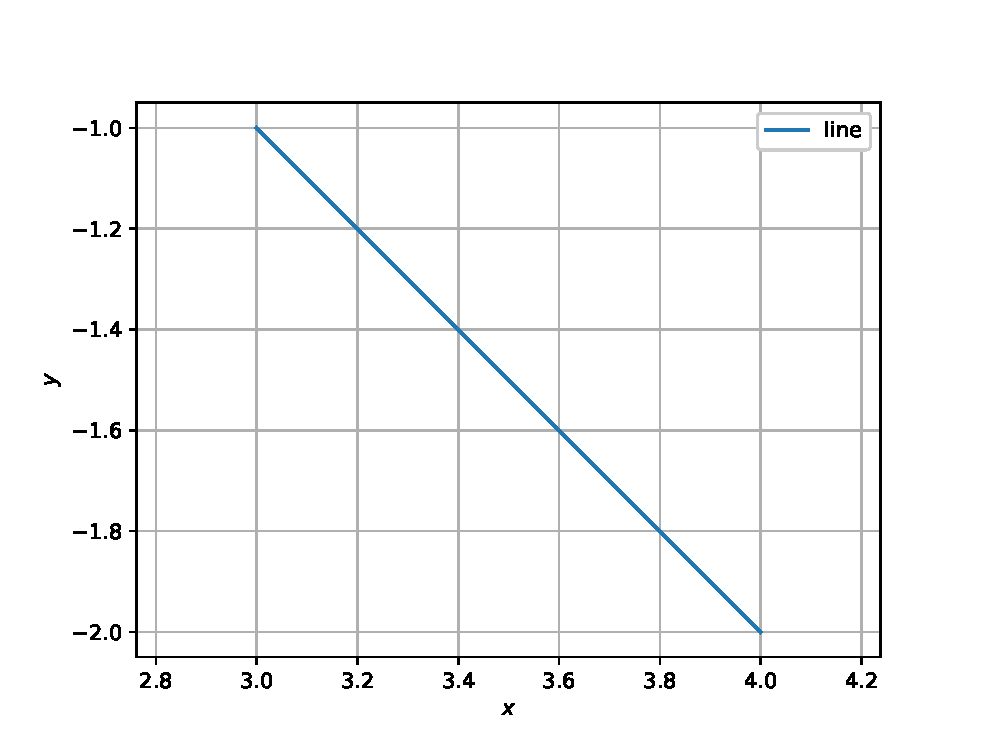
\includegraphics[width=\columnwidth]{./figs/lines/q9.eps}
	\caption{Line of Q.3.5.5}
	\label{fig:qnine}	
	\end{figure}
\end{comment}	
\end{enumerate}

